\section{FUNCTIONAL REQUIREMENTS}
\subsection{Actors}
\begin{itemize}
	\item \textbf{Fleet manager}, who performs the following activities:
	\begin{itemize}
		\item Login.
		\item Get bus location.
		\item Add/Remove/Modify fleet bus to the route.
		\item Add/Remove/Modify route.
		\item Add/Remove/Modify schedule time.
		\item Map the user requests.
		\item View previous user requests.
	\end{itemize}
\item \textbf{Bus driver}, who performs the following activities:
\begin{itemize}
	\item Login
	\item Handle user request
	\item View user request
	\item View schedule	
\end{itemize}
\item \textbf{Passenger}, who generates the user requests for a bus.
\end{itemize}
\newpage
\subsection{User stories and related requirements}
User stories are short and simple sentences that contain the features customers expect to find into the system. The customer\textquotesingle s requirements are not equally important; for this reason high, average or low priority is attributed to each of them.
\begin{table}[H]
	\centering
	\begin{tabular}{| m{2.2cm} | m{6cm} | m{1.5cm} | m{2.5cm} |}
		\hline
		\textbf{ID} & \textbf{User story} & \textbf{Priority} & \textbf{Use case}\\
		\hline
		UserStory1 & As fleet manager I want to be able to login (or logout) into the system with my account at any time. & High & \hyperlink{Login_fm}{Login}.\\
		\hline
		UserStory2 & As fleet manager I want to be able to add or remove a bus from a route. & High & \hyperlink{Add_bus_to_route_fm}{Add bus to route}. \hyperlink{Remove_bus_from_route_fm}{Remove bus from route}.\\
		\hline
		UserStory3 & As fleet manager I want to be able to add or remove a schedule time. & High & \hyperlink{Add_schedule_time_fm}{Add schedule time}. \hyperlink{Modify_schedule_time_fm}{Modify schedule time}.\\
		\hline
		UserStory4 & As fleet manager I want to be able to map user requests. & High & \hyperlink{Mapping_user_requests_fm}{Mapping user request}.\\
		\hline
		UserStory5 & As fleet manager I want to be able to add or modify a route. & High & \hyperlink{Add_route_fm}{Add route}. \hyperlink{Modify_route_fm}{Modify route}. \hyperlink{Delete_route_fm}{Delete route}.\\
		\hline
		UserStory6 & As fleet manager I want to be able to get the position of all the buses. & High & \hyperlink{Get_bus_location_fm}{Get bus location}.\\
		\hline
		UserStory7 & As fleet manager I want to be able to get the utilization of the selected bus. & Average & \hyperlink{View_bus_utilization_fm}{View bus utilization}.\\
		\hline
		UserStory8 & As a bus driver I want to be able to login (or logout) into the system with my account at any time. & High & \hyperlink{Login_bd}{Login}.\\
		\hline
		UserStory9 & As a bus driver I want to be able to see the schedule of the route I have to cover. & High & \hyperlink{View_schedule_bd}{View schedule}.\\
		\hline
		UserStory10 & As a bus driver I want to be able to view the user requests from the passengers. & Average & \hyperlink{View_user_requests_bd}{View user requests}.\\
		\hline
		UserStory11 & As a bus driver i want to be able to manage the user request. & High & \hyperlink{Manage_user_requests_bd}{Manage user requests}\\
		\hline
	\end{tabular}
\end{table}
\subsection{Use cases}
The following functional requirements describe the system’s behavior with respect to the BusPlanner project and its actors.
\begin{figure}[H]
	\centering
	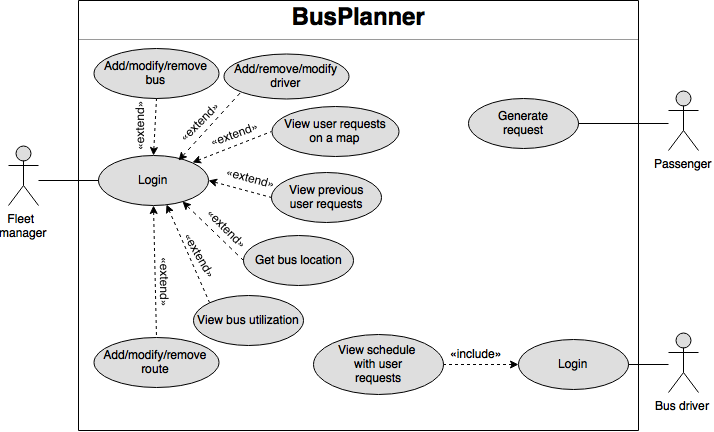
\includegraphics[width=15cm]{Use_cases}
	\caption{BusPlanner use case}
\end{figure}
\subsection{Use case description}
\subsubsection{Passenger}
\begin{table}[H]
	\centering
	\begin{tabular}{| m{3.5cm} | m{9.5cm} |}
		\hline
		\textbf{Name} & Generate request [\hyperlink{Generate_request}{Sequence diagram}]\\
		\hline
		\textbf{Actor} & Passenger\\
		\hline
		\textbf{Entry conditions} & Passenger is already known with the available buses on that route and all the necessary information.\\
		\hline
		\textbf{Flow of Events} & 
		\begin{enumerate}
			\item Check bus availability.
			\item See bus details for location.
			\item See bus schedule. 
			\item Make seat selection.
			\item Send location with timestamps.
		\end{enumerate}\\
		\hline
		\textbf{Exit Conditions} & Gets confirmation.\\
		\hline
		\textbf{Exceptions} & No bus/seat available.\\
		\hline
	\end{tabular}
\end{table}
\newpage
\subsubsection{Fleet manager}
\begin{itemize}
	\item \hypertarget{Login_fm} Login:
\begin{table}[H]
	\centering
	\begin{tabular}{| m{3.5cm} | m{9.5cm} |}
		\hline
		\textbf{Name} & Login [\hyperlink{Login_fm_seq}{Sequence diagram}]\\
		\hline
		\textbf{Actor} & Fleet manager\\
		\hline
		\textbf{Entry conditions} & The form is filled with credentials.\\
		\hline
		\textbf{Flow of Events} & 
		\begin{enumerate}
			\item Web page opened. 
			\item Enter the credentials.
			\item Enter button pressed.
		\end{enumerate}\\
		\hline
		\textbf{Exit Conditions} & Session variables.\\
		\hline
		\textbf{Exceptions} & Wrong credentials. Step is repeated.\\
		\hline
	\end{tabular}
\end{table}
\begin{figure}[H]
	\centering
	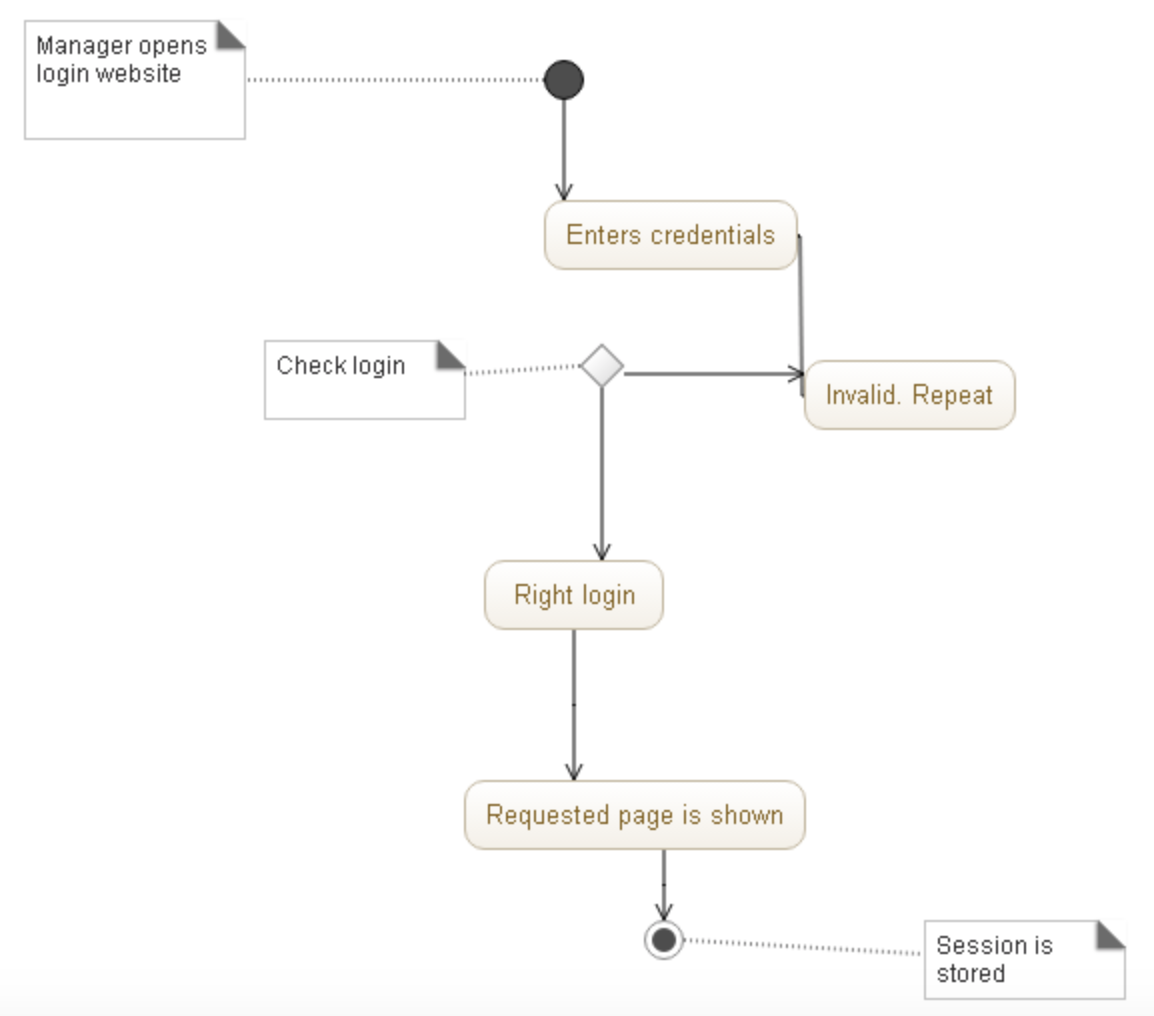
\includegraphics[height=13cm]{Login_fm}
\end{figure}
\item \hypertarget{Add_bus_to_route_fm} Add bus to route:
\begin{table}[H]
	\centering
	\begin{tabular}{| m{3.5cm} | m{9.5cm} |}
		\hline
		\textbf{Name} & Add bus to route [\hyperlink{Add_bus_to_route_fm_seq}{Sequence diagram}]\\
		\hline
		\textbf{Actor} & Fleet manager\\
		\hline
		\textbf{Entry conditions} & Fleet manager is logged in.\\
		\hline
		\textbf{Flow of Events} & 
		\begin{enumerate}
			\item Respective web page opened. 
			\item Respective form is filled with bus technical details. 
			\item Desired route and fleet selected. 
			\item Submit button pressed.
		\end{enumerate}\\
		\hline
		\textbf{Exit Conditions} & Database confirmation.\\
		\hline
		\textbf{Exceptions} & Wrong informations are inserted.\\
		\hline
	\end{tabular}
\end{table}
\begin{figure}[H]
	\centering
	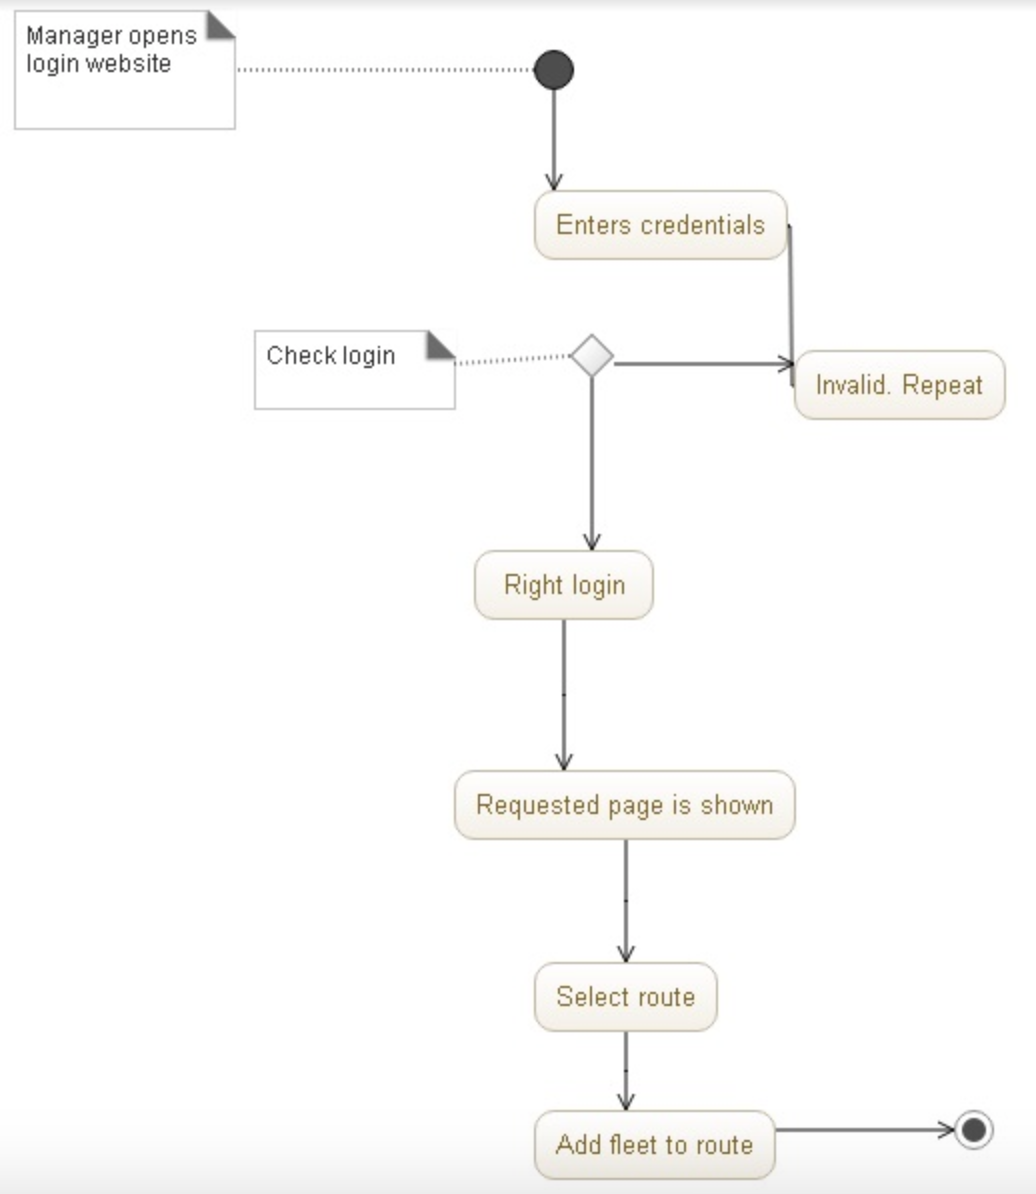
\includegraphics[height=12cm]{Add_bus_to_route_fm}
\end{figure}
\item \hypertarget{Remove_bus_from_route_fm} Remove bus from route:
\begin{table}[H]
	\centering
	\begin{tabular}{| m{3.5cm} | m{9.5cm} |}
		\hline
		\textbf{Name} & Remove bus from route [\hyperlink{Remove_bus_from_route_fm_seq}{Sequence diagram}]\\
		\hline
		\textbf{Actor} & Fleet manager\\
		\hline
		\textbf{Entry conditions} & Fleet manager is logged in.\\
		\hline
		\textbf{Flow of Events} & 
		\begin{enumerate}
			\item Respective web page is opened.  
			\item Desired route and fleet selected. 
			\item Information is shown on map. 
			\item Bus is removed from the route.
		\end{enumerate}\\
		\hline
		\textbf{Exit Conditions} & The schedule is affected.\\
		\hline
		\textbf{Exceptions} & Bus not found.\\
		\hline
	\end{tabular}
\end{table}
\begin{figure}[H]
	\centering
	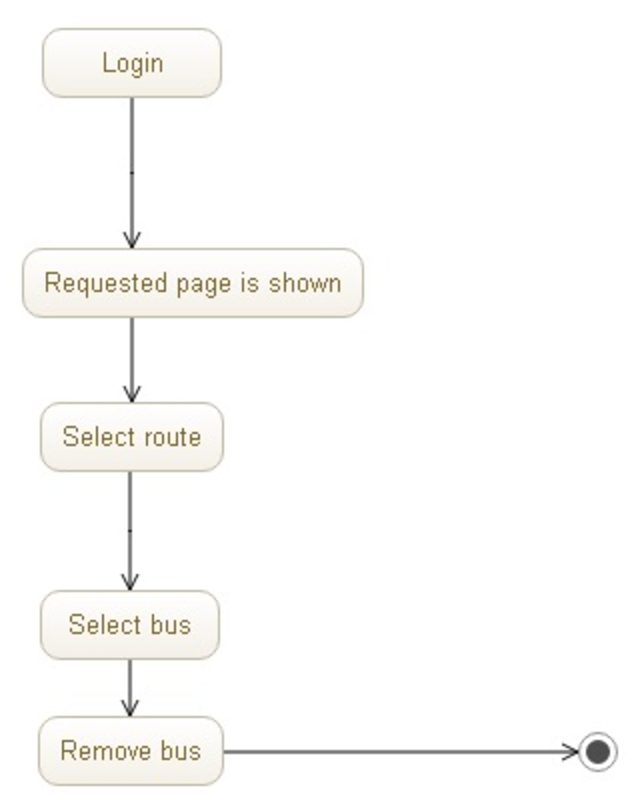
\includegraphics[height=13cm]{Remove_bus_from_route_fm}
\end{figure}
\item \hypertarget{Add_schedule_time_fm} Add schedule time:
\begin{table}[H]
	\centering
	\begin{tabular}{| m{3.5cm} | m{9.5cm} |}
		\hline
		\textbf{Name} & Add schedule time [\hyperlink{Add_schedule_time_fm_seq}{Sequence diagram}]\\
		\hline
		\textbf{Actor} & Fleet manager\\
		\hline
		\textbf{Entry conditions} & Fleet manager is logged in.\\
		\hline
		\textbf{Flow of Events} & 
		\begin{enumerate}
			\item Respective web page is opened. 
			\item Desired route is selected. 
			\item Information is shown on the map. 
			\item Schedule form is filled.
		\end{enumerate}\\
		\hline
		\textbf{Exit Conditions} & The database is updated.\\
		\hline
		\textbf{Exceptions} & The driver cannot see the schedule.\\
		\hline
	\end{tabular}
\end{table}
\begin{figure}[H]
	\centering
	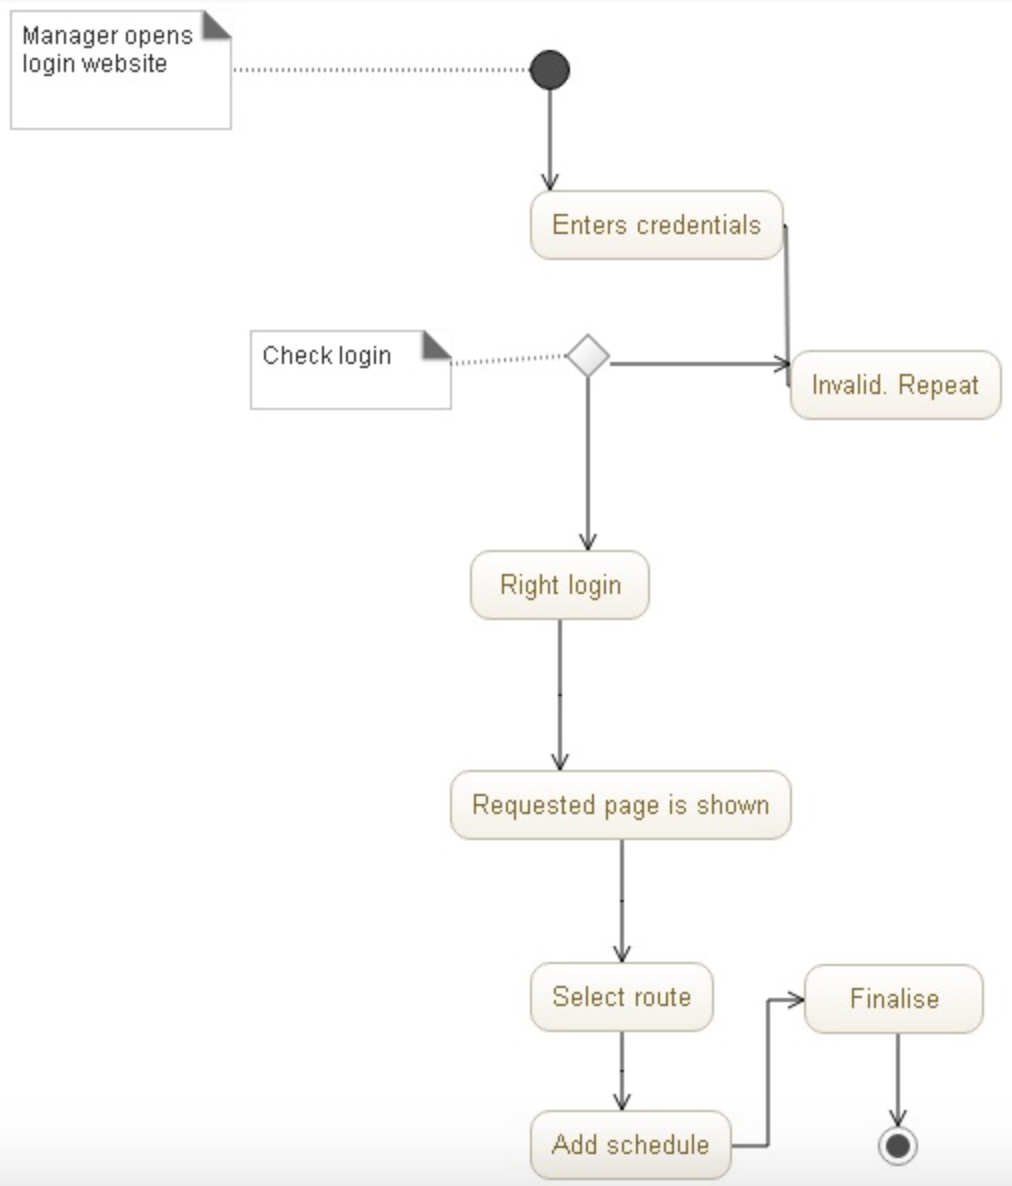
\includegraphics[height=13cm]{Add_schedule_time_fm}
\end{figure}
\item \hypertarget{Modify_schedule_time_fm} Modify schedule time:
\begin{table}[H]
	\centering
	\begin{tabular}{| m{3.5cm} | m{9.5cm} |}
		\hline
		\textbf{Name} & Modify schedule time [\hyperlink{Modify_schedule_time_fm_seq}{Sequence diagram}]\\
		\hline
		\textbf{Actor} & Fleet manager\\
		\hline
		\textbf{Entry conditions} & Fleet manager is logged in.\\
		\hline
		\textbf{Flow of Events} & 
		\begin{enumerate}
			\item Respective web page is opened. 
			\item Desired schedule is selected. 
			\item Information is shown. 
			\item Schedule form is filled.
		\end{enumerate}\\
		\hline
		\textbf{Exit Conditions} & The database is updated.\\
		\hline
		\textbf{Exceptions} & The driver cannot see the schedule.\\
		\hline
	\end{tabular}
\end{table}
\begin{figure}[H]
	\centering
	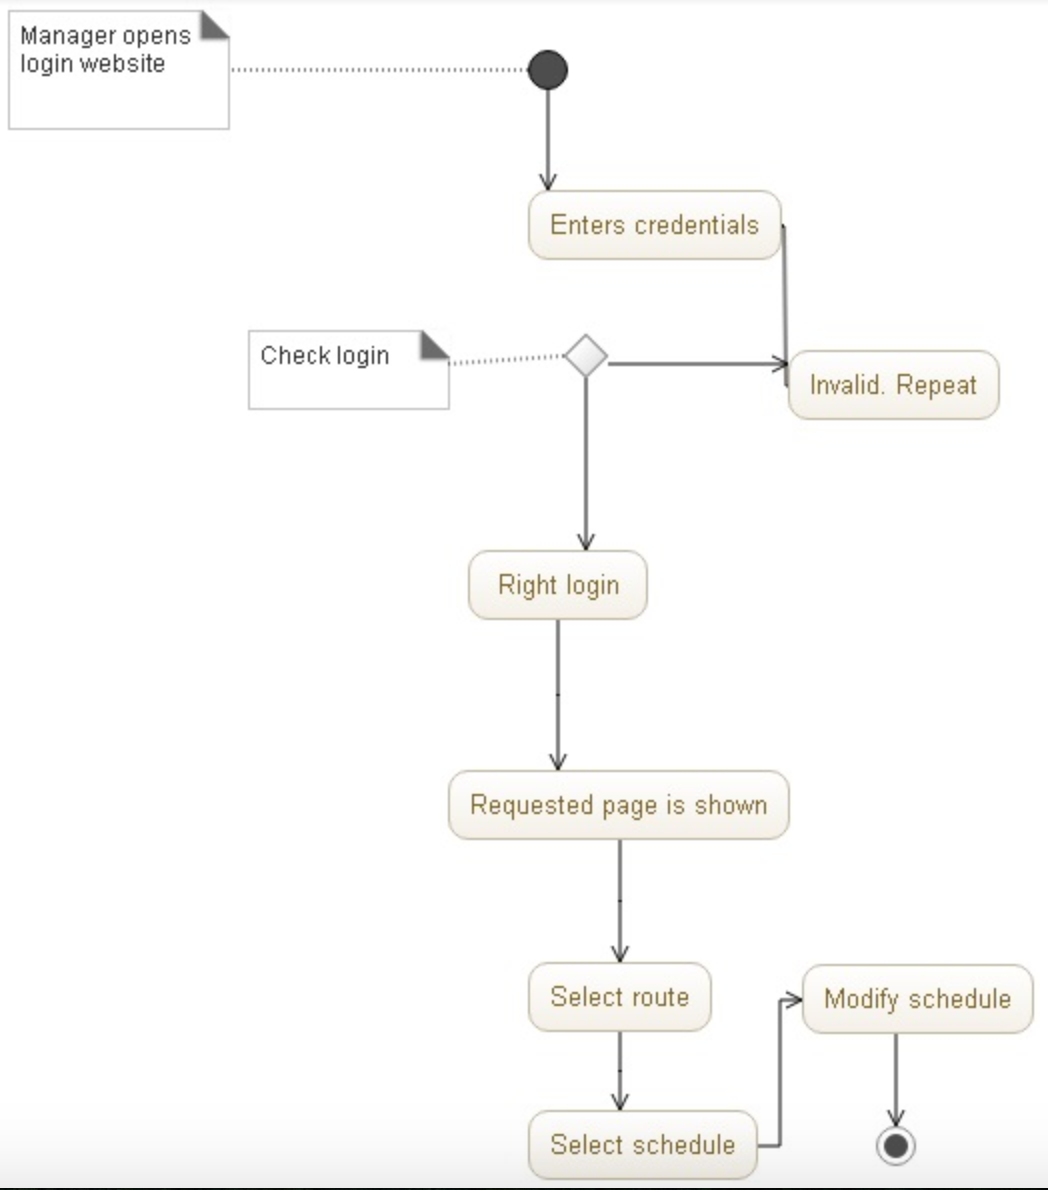
\includegraphics[height=13cm]{Modify_schedule_time_fm}
\end{figure}
\item \hypertarget{Mapping_user_requests_fm} Mapping user requests:
\begin{table}[H]
	\centering
	\begin{tabular}{| m{3.5cm} | m{9.5cm} |}
		\hline
		\textbf{Name} & Mapping user requests [\hyperlink{Mapping_user_requests_fm_seq}{Sequence diagram}]\\
		\hline
		\textbf{Actor} & Fleet manager\\
		\hline
		\textbf{Entry conditions} & Fleet manager is logged in.\\
		\hline
		\textbf{Flow of Events} & 
		\begin{enumerate}
			\item Respective web page is opened. 
			\item Read from database. 
			\item Information is shown.
		\end{enumerate}\\
		\hline
		\textbf{Exit Conditions} & The database is updated.\\
		\hline
		\textbf{Exceptions} & Data is not available.\\
		\hline
	\end{tabular}
\end{table}
\begin{figure}[H]
	\centering
	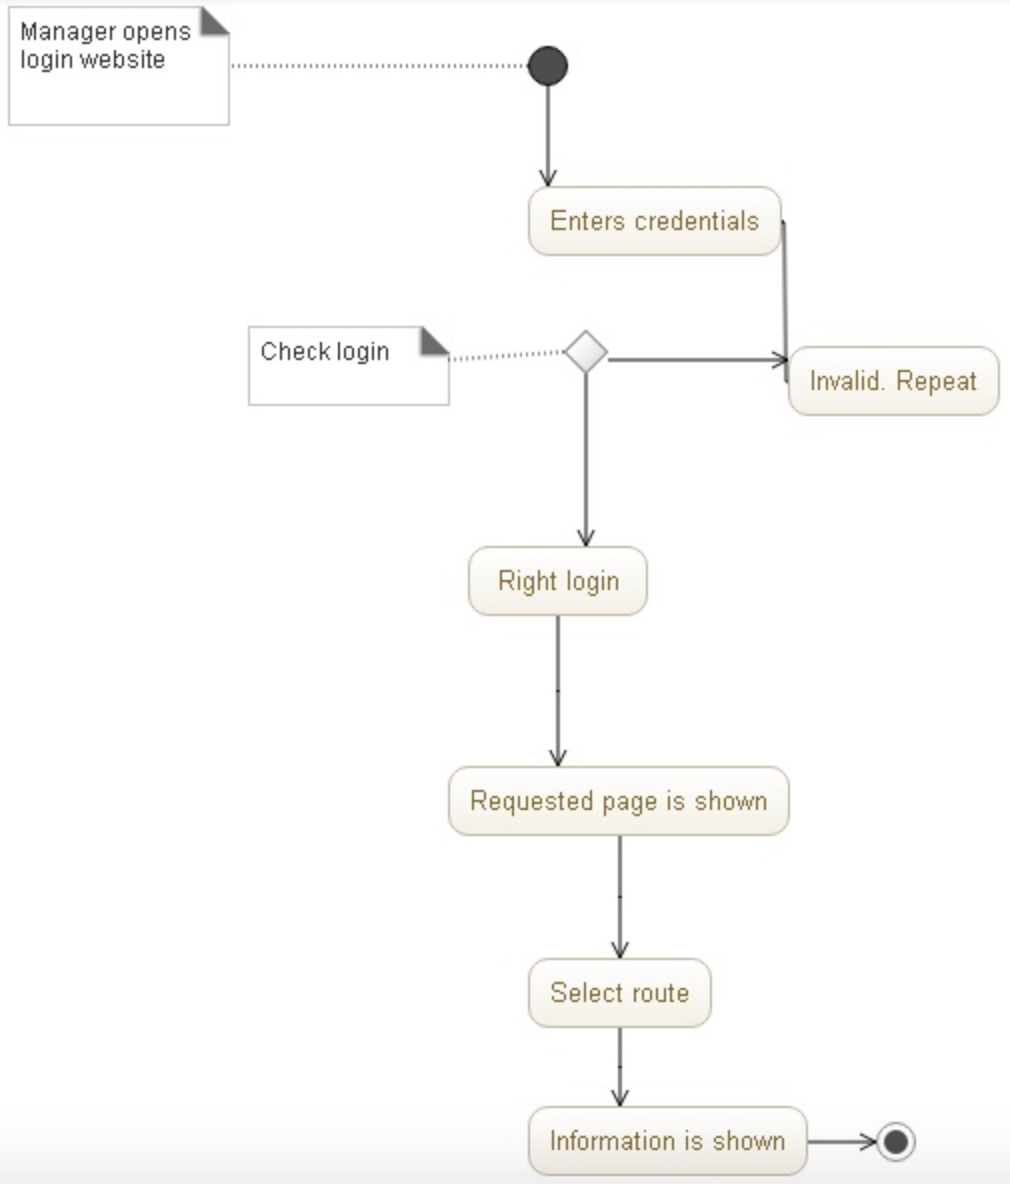
\includegraphics[height=13cm]{Mapping_user_requests_fm}
\end{figure}
\item \hypertarget{View_previous_user_requests_fm} View previous user requests:
\begin{table}[H]
	\centering
	\begin{tabular}{| m{3.5cm} | m{9.5cm} |}
		\hline
		\textbf{Name} & View previous user requests [\hyperlink{View_previous_user_requests_fm_seq}{Sequence diagram}]\\
		\hline
		\textbf{Actor} & Fleet manager\\
		\hline
		\textbf{Entry conditions} & Fleet manager is logged in.\\
		\hline
		\textbf{Flow of Events} & 
		\begin{enumerate}
			\item Respective web page is opened. 
			\item Previous user requests are selected. 
			\item Read data from the database.
			\item Information is shown. 
		\end{enumerate}\\
		\hline
		\textbf{Exit Conditions} & Getting previous users requests.\\
		\hline
		\textbf{Exceptions} & Data is not available.\\
		\hline
	\end{tabular}
\end{table}
\begin{figure}[H]
	\centering
	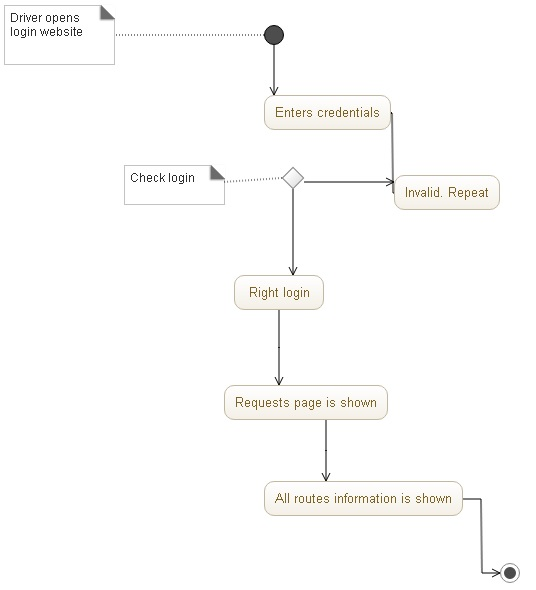
\includegraphics[height=13cm]{View_previous_user_requests_fm}
\end{figure}
\newpage
\item \hypertarget{Add_route_fm} Add route:
\begin{table}[H]
	\centering
	\begin{tabular}{| m{3.5cm} | m{9.5cm} |}
		\hline
		\textbf{Name} & Add route [\hyperlink{Add_route_fm_seq}{Sequence diagram}]\\
		\hline
		\textbf{Actor} & Fleet manager\\
		\hline
		\textbf{Entry conditions} & Fleet manager is logged in.\\
		\hline
		\textbf{Flow of Events} & 
		\begin{enumerate}
			\item Respective web page is opened. 
			\item Desired route information is filled.  
			\item Submit button is pressed.
		\end{enumerate}\\
		\hline
		\textbf{Exit Conditions} & The database is updated.\\
		\hline
		\textbf{Exceptions} & The database is not updated.\\
		\hline
	\end{tabular}
\end{table}
\begin{figure}[H]
	\centering
	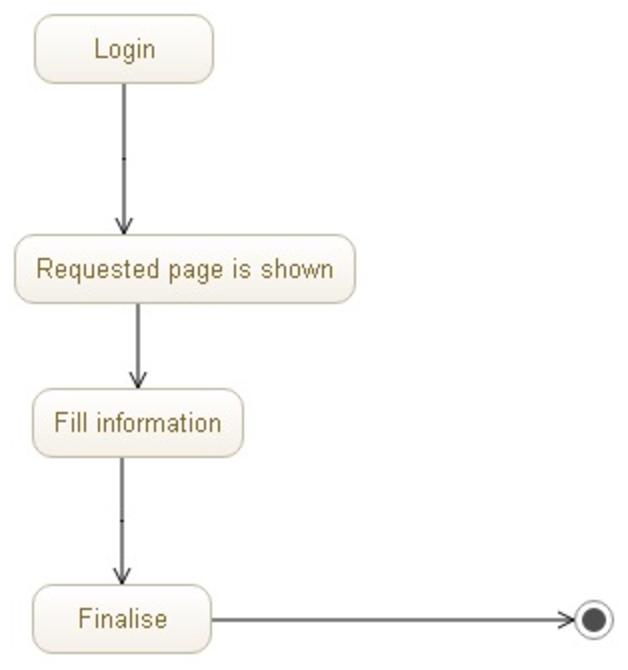
\includegraphics[height=13cm]{Add_route_fm}
\end{figure}
\item \hypertarget{Modify_route_fm} Modify route:
\begin{table}[H]
	\centering
	\begin{tabular}{| m{3.5cm} | m{9.5cm} |}
		\hline
		\textbf{Name} & Modify route [\hyperlink{Modify_route_fm_seq}{Sequence diagram}]\\
		\hline
		\textbf{Actor} & Fleet manager\\
		\hline
		\textbf{Entry conditions} & Fleet manager is logged in.\\
		\hline
		\textbf{Flow of Events} & 
		\begin{enumerate}
			\item Respective web page is opened. 
			\item Desired route information is modified.  
			\item Submit button is pressed.
		\end{enumerate}\\
		\hline
		\textbf{Exit Conditions} & The database is updated.\\
		\hline
		\textbf{Exceptions} & The database is not updated.\\
		\hline
	\end{tabular}
\end{table}
\begin{figure}[H]
	\centering
	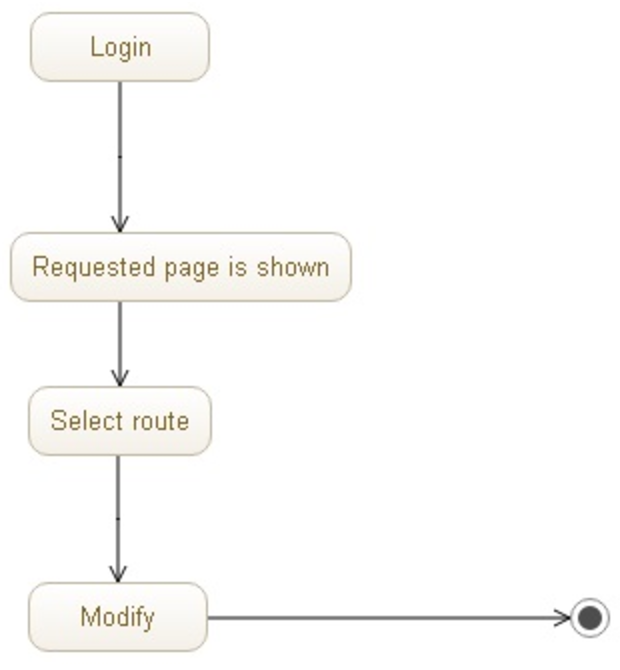
\includegraphics[height=13cm]{Modify_route_fm}
\end{figure}
\item \hypertarget{Delete_route_fm} Delete route:
\begin{table}[H]
	\centering
	\begin{tabular}{| m{3.5cm} | m{9.5cm} |}
		\hline
		\textbf{Name} & Delete route [\hyperlink{Delete_route_fm_seq}{Sequence diagram}]\\
		\hline
		\textbf{Actor} & Fleet manager\\
		\hline
		\textbf{Entry conditions} & Fleet manager is logged in.\\
		\hline
		\textbf{Flow of Events} & 
		\begin{enumerate}
			\item Respective web page is opened. 
			\item Desired route information is deleted.  
			\item Submit button is pressed.
		\end{enumerate}\\
		\hline
		\textbf{Exit Conditions} & The database is updated.\\
		\hline
		\textbf{Exceptions} & The database is not updated.\\
		\hline
	\end{tabular}
\end{table}
\begin{figure}[H]
	\centering
	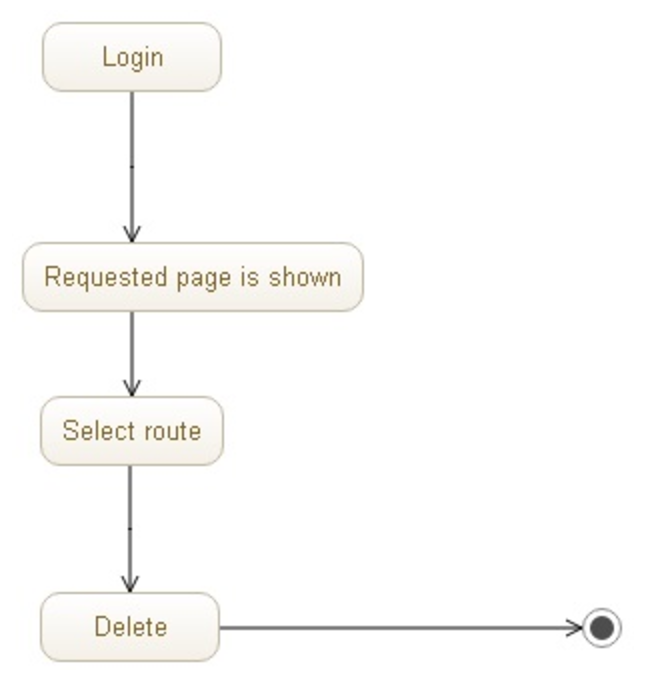
\includegraphics[height=13.5cm]{Delete_route_fm}
\end{figure}
\item \hypertarget{Get_bus_location_fm} Get bus location:
\begin{table}[H]
	\centering
	\begin{tabular}{| m{3.5cm} | m{9.5cm} |}
		\hline
		\textbf{Name} & Get bus location [\hyperlink{Get_bus_location_fm_seq}{Sequence diagram}]\\
		\hline
		\textbf{Actor} & Fleet manager\\
		\hline
		\textbf{Entry conditions} & Fleet manager is logged in.\\
		\hline
		\textbf{Flow of Events} & 
		\begin{enumerate}
			\item Respective web page is opened. 
			\item Desired bus is selected. 
			\item Information is shown in the map.
		\end{enumerate}\\
		\hline
		\textbf{Exit Conditions} & Getting the bus\textquotesingle s current position in map.\\
		\hline
		\textbf{Exceptions} & Data not available.\\
		\hline
	\end{tabular}
\end{table}
\begin{figure}[H]
	\centering
	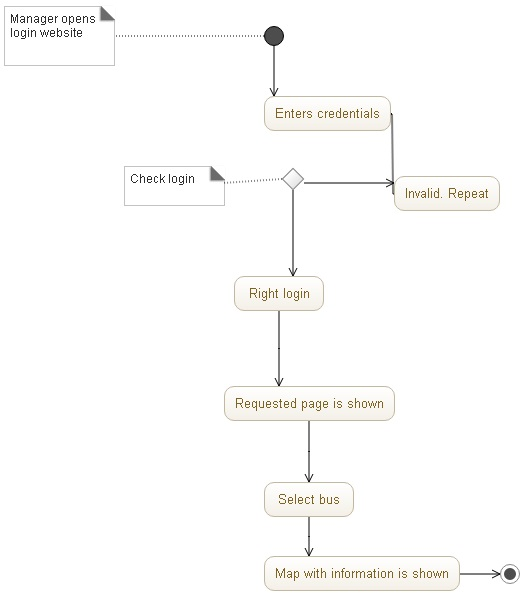
\includegraphics[height=13.5cm]{Get_bus_location_fm}
\end{figure}
\item \hypertarget{View_bus_utilization_fm} View bus utilization:
\begin{table}[H]
	\centering
	\begin{tabular}{| m{3.5cm} | m{9.5cm} |}
		\hline
		\textbf{Name} & View bus utilization [\hyperlink{View_bus_utilization_fm_seq}{Sequence diagram}]\\
		\hline
		\textbf{Actor} & Fleet manager\\
		\hline
		\textbf{Entry conditions} & Fleet manager is logged in.\\
		\hline
		\textbf{Flow of Events} & 
		\begin{enumerate}
			\item Respective web page is opened. 
			\item Desired bus is selected. 
			\item Information is shown.
		\end{enumerate}\\
		\hline
		\textbf{Exit Conditions} & Getting the utilization of buses.\\
		\hline
		\textbf{Exceptions} & Data not available.\\
		\hline
	\end{tabular}
\end{table}
\begin{figure}[H]
	\centering
	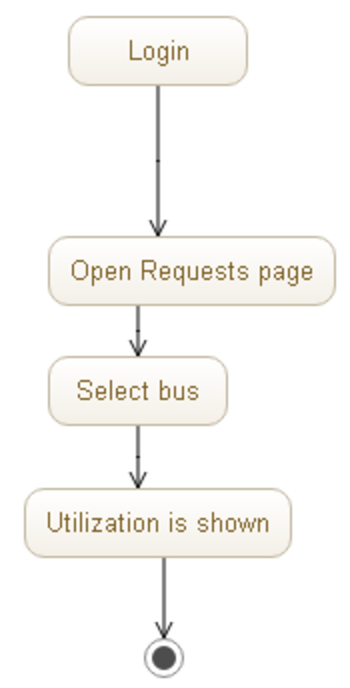
\includegraphics[height=13.5cm]{View_bus_utilization_fm}
\end{figure}
\end{itemize}
\subsubsection{Bus driver}
\begin{itemize}
	\item \hypertarget{Login_bd} Login:
	\begin{table}[H]
		\centering
		\begin{tabular}{| m{3.5cm} | m{9.5cm} |}
			\hline
			\textbf{Name} & Login [\hyperlink{Login_bd_seq}{Sequence diagram}]\\
			\hline
			\textbf{Actor} & Bus driver\\
			\hline
			\textbf{Entry conditions} & Form is filled with credentials.\\
			\hline
			\textbf{Flow of Events} & 
			\begin{enumerate}
				\item Web page is opened. 
				\item Form is filled. 
				\item Enter button pressed.
			\end{enumerate}\\
			\hline
			\textbf{Exit Conditions} & Session variables.\\
			\hline
			\textbf{Exceptions} & Wrong credentials. Step is repeated.\\
			\hline
		\end{tabular}
	\end{table}
\begin{figure}[H]
	\centering
	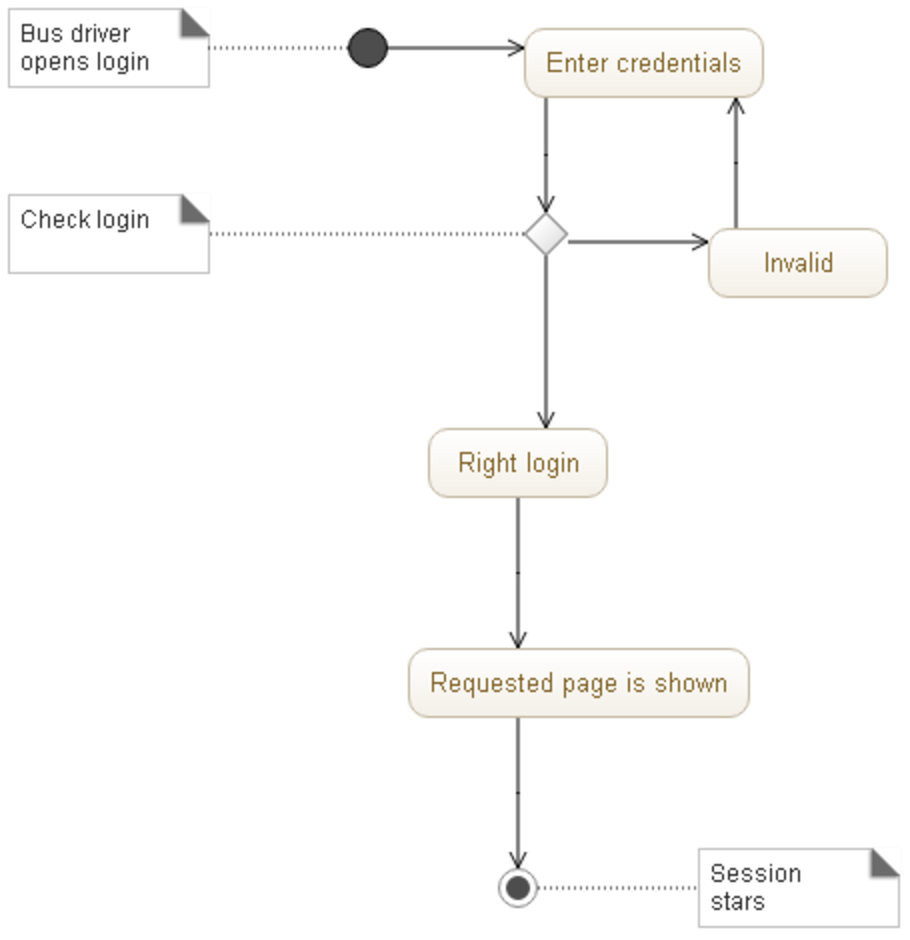
\includegraphics[width=15cm]{Login_bd}
\end{figure}
	\item \hypertarget{View_schedule_bd} View schedule:
	\begin{table}[H]
		\centering
		\begin{tabular}{| m{3.5cm} | m{9.5cm} |}
			\hline
			\textbf{Name} & View schedule [\hyperlink{View_schedule_bd_seq}{Sequence diagram}]\\
			\hline
			\textbf{Actor} & Bus driver\\
			\hline
			\textbf{Entry conditions} & Bus driver is logged in.\\
			\hline
			\textbf{Flow of Events} & 
			\begin{enumerate}
				\item Respective web page is opened. 
				\item Read data from database. 
				\item Information is shown in the screen.
			\end{enumerate}\\
			\hline
			\textbf{Exit Conditions} & Getting the schedule.\\
			\hline
			\textbf{Exceptions} & Data not available.\\
			\hline
		\end{tabular}
	\end{table}
\begin{figure}[H]
	\centering
	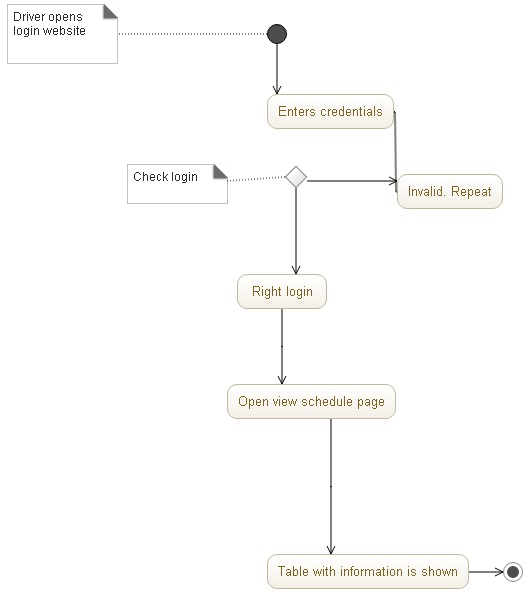
\includegraphics[height=13.5cm]{View_schedule_bd}
\end{figure}
\newpage
	\item \hypertarget{View_user_requests_bd} View user requests:
	\begin{table}[H]
		\centering
		\begin{tabular}{| m{3.5cm} | m{9.5cm} |}
			\hline
			\textbf{Name} & View user requests [\hyperlink{View_user_requests_bd_seq}{Sequence diagram}]\\
			\hline
			\textbf{Actor} & Bus driver\\
			\hline
			\textbf{Entry conditions} & Bus driver is logged in.\\
			\hline
			\textbf{Flow of Events} & 
			\begin{enumerate}
				\item Respective web page is opened. 
				\item Desired user is selected. 
				\item Read data from the database. 
				\item Information is shown on the screen.
			\end{enumerate}\\
			\hline
			\textbf{Exit Conditions} & Getting the user\textquotesingle s requests.\\
			\hline
			\textbf{Exceptions} & Data not available.\\
			\hline
		\end{tabular}
	\end{table}
\begin{figure}[H]
	\centering
	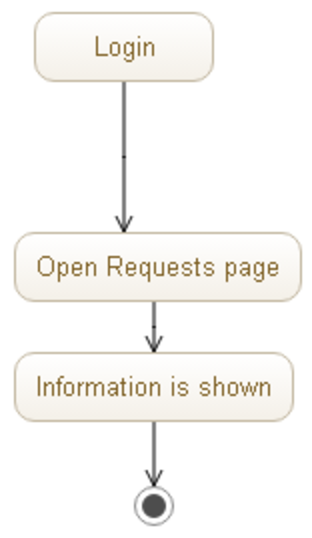
\includegraphics[height=13cm]{View_user_requests_bd}
\end{figure}
	\item \hypertarget{Manage_user_requests_bd} Manage user requests:
	\begin{table}[H]
		\centering
		\begin{tabular}{| m{3.5cm} | m{9.5cm} |}
			\hline
			\textbf{Name} & Manage user requests [\hyperlink{Manage_user_requests_bd_seq}{Sequence diagram}]\\
			\hline
			\textbf{Actor} & Bus driver\\
			\hline
			\textbf{Entry conditions} & Bus driver is logged in.\\
			\hline
			\textbf{Flow of Events} & 
			\begin{enumerate}
				\item Respective web page is opened. 
				\item Desired user selected. 
				\item Desired request is managed. 
				\item Submit button is pressed.
			\end{enumerate}\\
			\hline
			\textbf{Exit Conditions} & Database is updated.\\
			\hline
			\textbf{Exceptions} & Database is not updated.\\
			\hline
		\end{tabular}
	\end{table}
\begin{figure}[H]
	\centering
	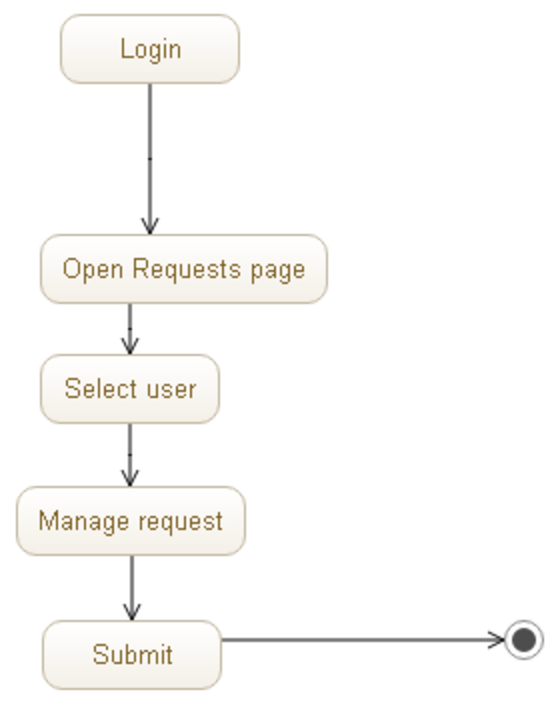
\includegraphics[height=13cm]{Manage_user_requests_bd}
\end{figure}
\end{itemize}
\newpage
\subsubsection{Sequence diagrams}
\begin{itemize}
	\item \hypertarget{Generate_request} Generate request:
	\begin{figure}[H]
		\centering
		\includegraphics[height=19cm]{Generate_request}
	\end{figure}
	\item \hypertarget{Login_fm_seq} Fleet manager login:
	\begin{figure}[H]
		\centering
		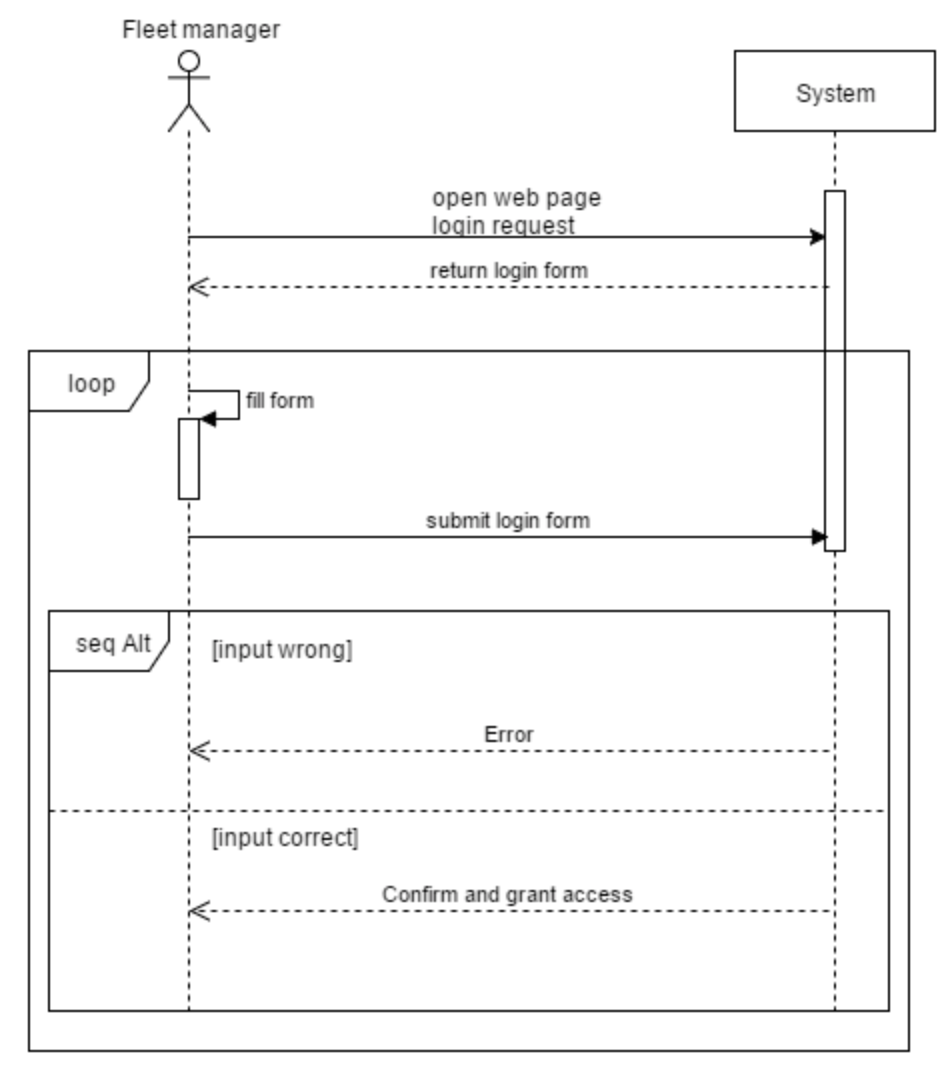
\includegraphics[width=13cm]{Login_fm_seq}
	\end{figure}
\newpage
	\item \hypertarget{Add_bus_to_route_fm_seq} Add bus to route:
	\begin{figure}[H]
		\centering
		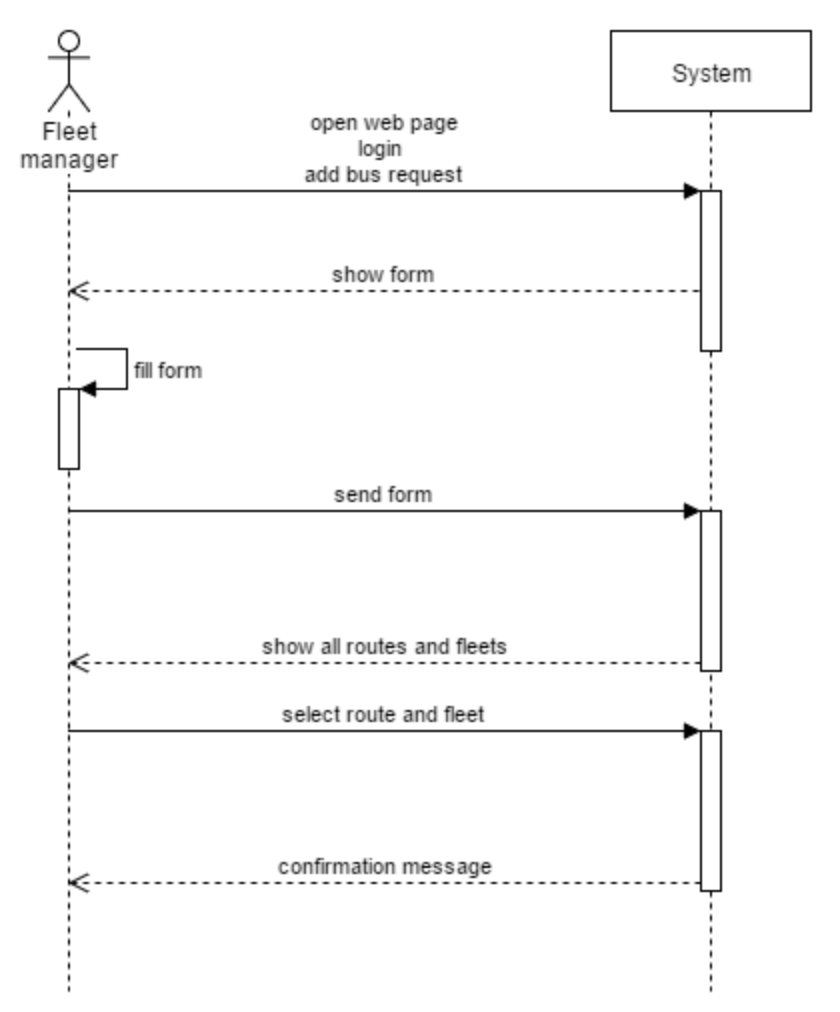
\includegraphics[width=13cm]{Add_bus_to_route_fm_seq}
	\end{figure}
\newpage
\item \hypertarget{Remove_bus_from_route_fm_seq} Remove bus from route:
\begin{figure}[H]
	\centering
	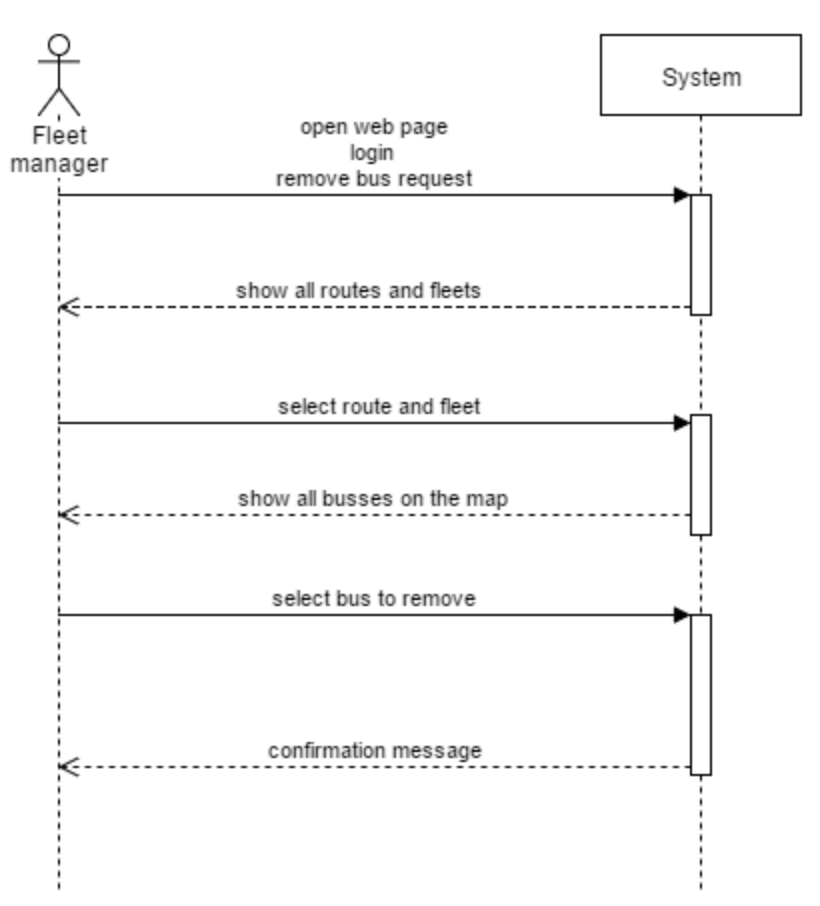
\includegraphics[width=13cm]{Remove_bus_from_route_fm_seq}
\end{figure}
\newpage
\item \hypertarget{Add_schedule_time_fm_seq} Add schedule time:
\begin{figure}[H]
	\centering
	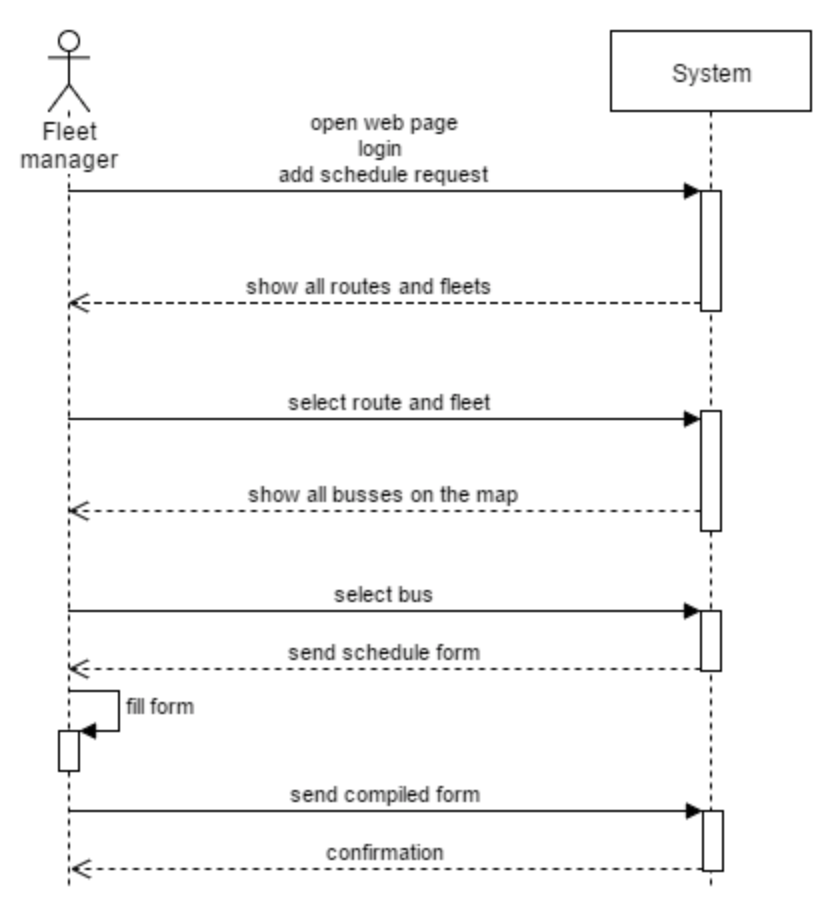
\includegraphics[width=13cm]{Add_schedule_time_fm_seq}
\end{figure}
\newpage
\item \hypertarget{Modify_schedule_time_fm_seq} Modify schedule time:
\begin{figure}[H]
	\centering
	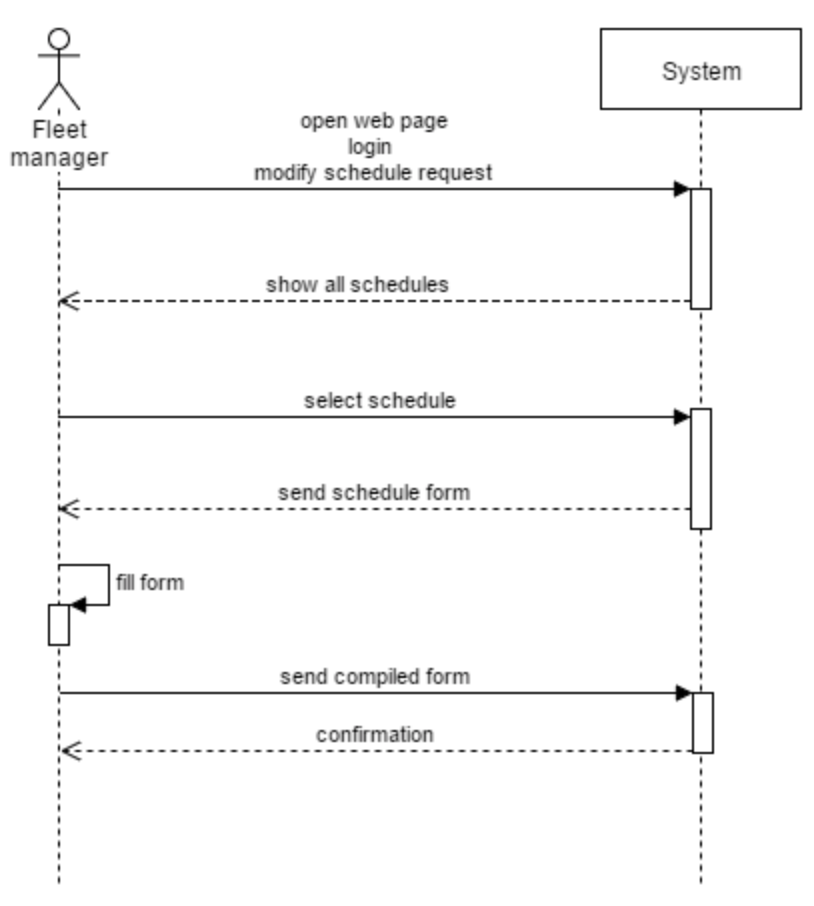
\includegraphics[width=13cm]{Modify_schedule_time_fm_seq}
\end{figure}
\newpage
\item \hypertarget{Mapping_user_requests_fm_seq} Mapping user requests:
\begin{figure}[H]
	\centering
	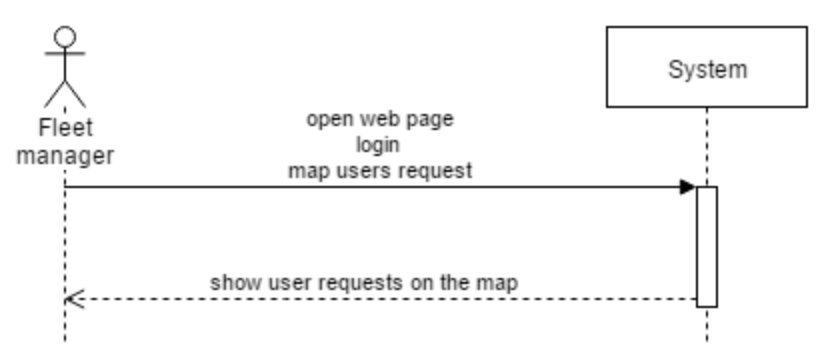
\includegraphics[width=13cm]{Mapping_user_requests_fm_seq}
\end{figure}
\item \hypertarget{View_previous_user_requests_fm_seq} View previous user requests:
\begin{figure}[H]
	\centering
	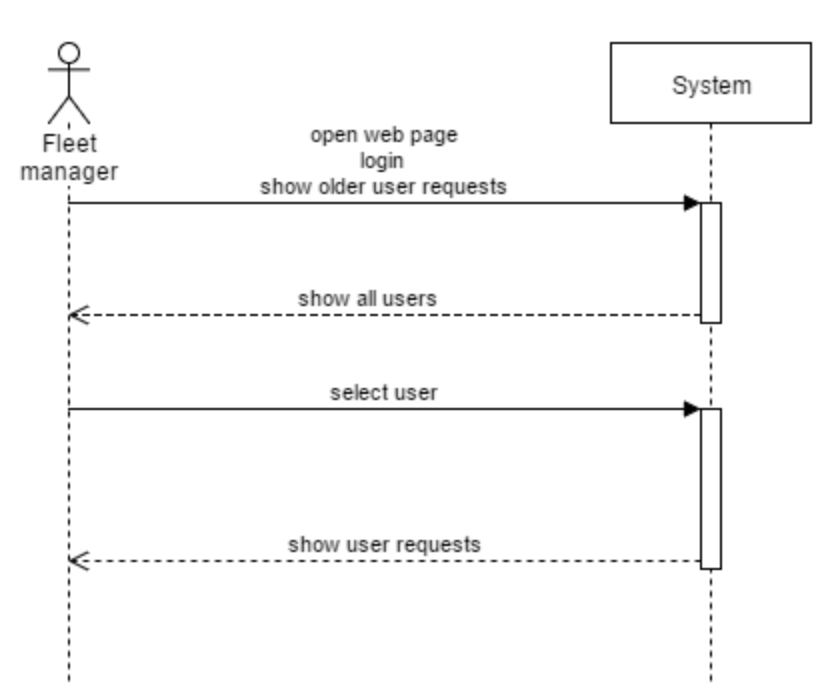
\includegraphics[height=12cm]{View_previous_user_requests_fm_seq}
\end{figure}
\item \hypertarget{Add_route_fm_seq} Add route:
\begin{figure}[H]
	\centering
	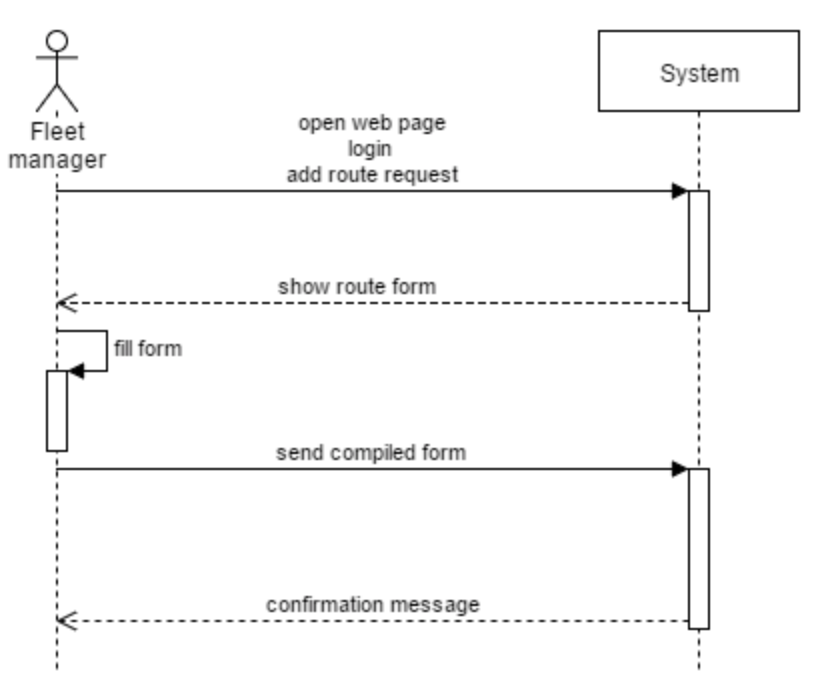
\includegraphics[width=13cm]{Add_route_fm_seq}
\end{figure}
\newpage
\item \hypertarget{Modify_route_fm_seq} Modify route:
\begin{figure}[H]
	\centering
	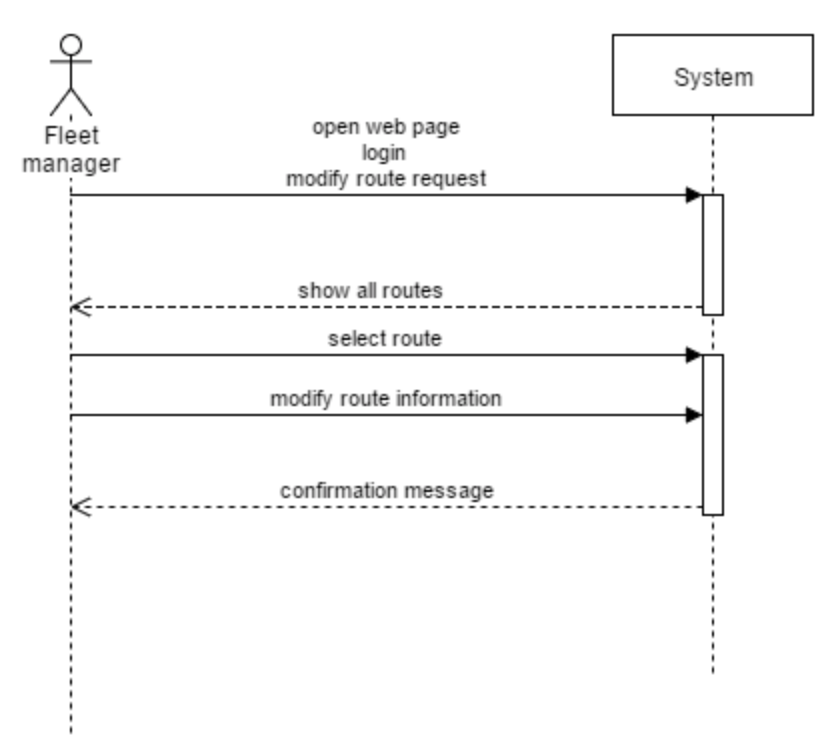
\includegraphics[width=13cm]{Modify_route_fm_seq}
\end{figure}
\newpage
\item \hypertarget{Delete_route_fm_seq} Delete route:
\begin{figure}[H]
	\centering
	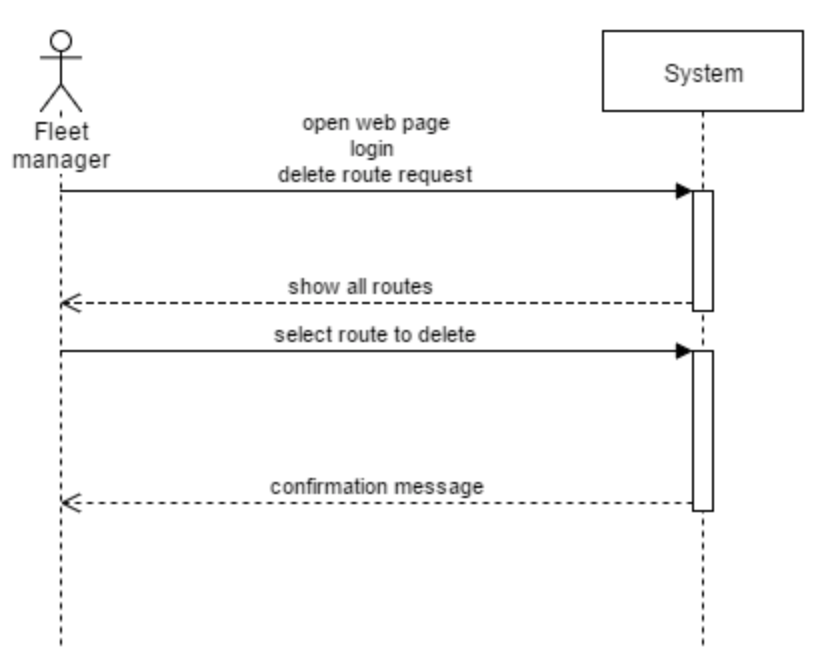
\includegraphics[width=13cm]{Delete_route_fm_seq}
\end{figure}
\newpage
\item \hypertarget{Get_bus_location_fm_seq} Get bus location:
\begin{figure}[H]
	\centering
	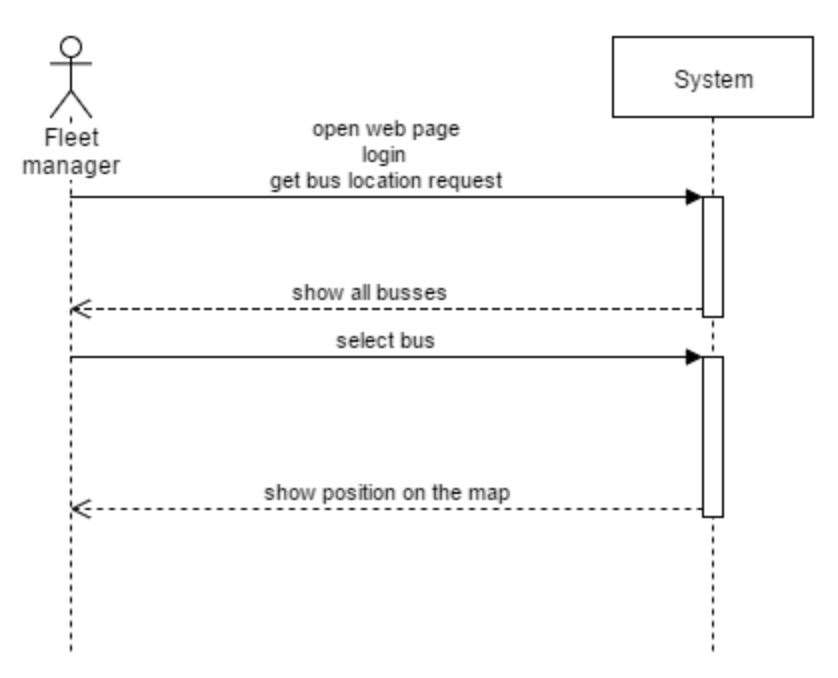
\includegraphics[width=13cm]{Get_bus_location_fm_seq}
\end{figure}
\newpage
\item \hypertarget{View_bus_utilization_fm_seq} View bus utilization:
\begin{figure}[H]
	\centering
	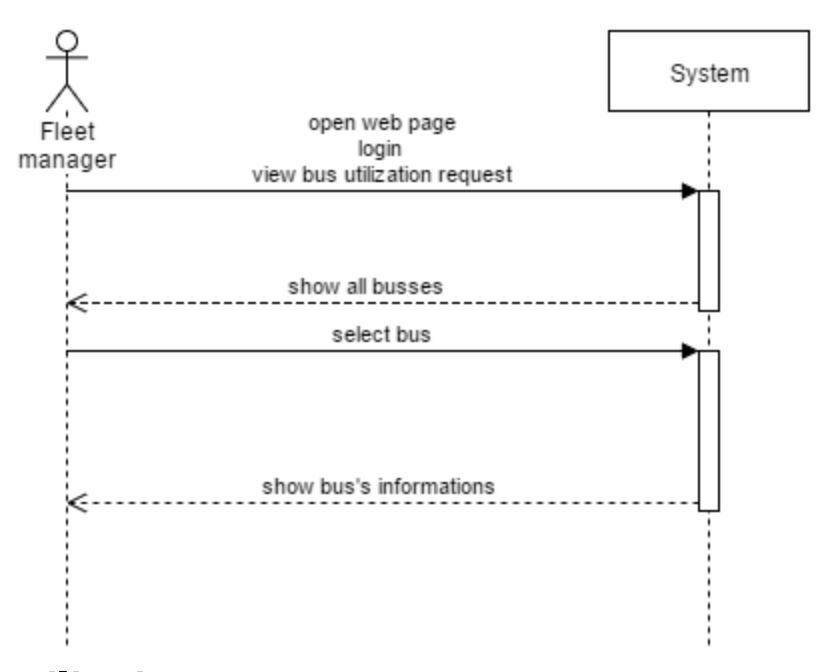
\includegraphics[width=13cm]{View_bus_utilization_fm_seq}
\end{figure}
\newpage
\item \hypertarget{Add_notification_for_drivers_fm_seq} Add notification for drivers:
\begin{figure}[H]
	\centering
	\includegraphics[width=13cm]{Add_notification_for_drivers_fm_seq}
\end{figure}
\newpage
\item \hypertarget{Control_vehicle_status_fm_seq} Control vehicle status:
\begin{figure}[H]
	\centering
	\includegraphics[width=13cm]{Control_vehicle_status_fm_seq}
\end{figure}
\newpage
\item \hypertarget{Update_fleet_information_fm_seq} Update fleet information:
\begin{figure}[H]
	\centering
	\includegraphics[width=13cm]{Update_fleet_information_fm_seq}
\end{figure}
\newpage
\item \hypertarget{Login_bd_seq} Bus driver login:
\begin{figure}[H]
	\centering
	\includegraphics[width=13cm]{Login_bd_seq}
\end{figure}
\newpage
\item \hypertarget{View_schedule_bd_seq} View schedule:
\begin{figure}[H]
	\centering
	\includegraphics[width=13cm]{View_schedule_bd_seq}
\end{figure}
\newpage
\item \hypertarget{View_user_requests_bd_seq} View user requests:
\begin{figure}[H]
	\centering
	\includegraphics[width=13cm]{View_user_requests_bd_seq}
\end{figure}
\newpage
\item \hypertarget{Manage_user_requests_bd_seq} Manage user requests:
\begin{figure}[H]
	\centering
	\includegraphics[width=13cm]{Manage_user_requests_bd_seq}
\end{figure}
\end{itemize}